\documentclass[11pt,a4paper]{article}
\usepackage[T1]{fontenc}
\usepackage{lmodern,microtype,amsmath,booktabs,tabularx,array,graphicx}
\usepackage{float}
\usepackage{pgfplots}
\pgfplotsset{compat=1.18}
\usepackage[margin=21mm]{geometry}
\usepackage[colorlinks=true,linkcolor=blue,urlcolor=blue]{hyperref}
\setlength{\parindent}{0pt}
\setlength{\parskip}{7pt}
\setlength{\emergencystretch}{2em}
\newcolumntype{Y}{>{\raggedright\arraybackslash}X}
\newcommand{\mase}{\operatorname{MASE}}
\newcommand{\smase}{\operatorname{sMASE}}
\newcommand{\mae}{\operatorname{MAE}}
\newcommand{\featurecode}[2]{\href{https://github.com/3gaspo/evaluating_tsfms/blob/c119ed748d149e9f7892641bead393819f5983fd/src/timebench/feature/features.py\#L#1}{#2}}
\title{\textbf{Evaluating Time-Series Foundation Models}\\Scientific Executive Summary}
\author{}
\date{21 September 2026; results computed 17--21 September 2026}
\begin{document}
\begin{center}
{\Large\bfseries Evaluating Time-Series Foundation Models}\\[4pt]
{\large Scientific Executive Summary}\\[5pt]
{\small 21 September 2026; results computed 17--21 September 2026}
\end{center}

\section*{Main findings}
\begin{itemize}
\item \textbf{Foundation models:} Chronos-2 achieves scaled MASE 0.6855
and wins 74 of 98 matched TIME tasks, ahead of TS-ICL and Chronos-Bolt.
It also has the lowest measured total forecasting time (439.1 seconds).
\item \textbf{Channel representation:} native multivariate Chronos-2 is
0.8\% better in aggregate than independent univariate forecasting.
Recasting other target histories as past covariates gives essentially the
same accuracy as native input, with 5.68 times its measured forecasting time.
\item \textbf{Dataset features:} greater temporal heterogeneity accompanies
higher scaled MASE for all three foundation models, with Spearman rank
correlations of 0.42--0.50 across the 50 configurations.
\item \textbf{Context length:} Chronos-2 at 4,096 input steps has sMASE
0.6824, 0.45\% lower than at 8,192, with 40.7\% less recorded forecasting
time. Halving the maximum context costs 1.34\% sMASE for Chronos-Bolt and
0.21\% for TS-ICL, while reducing time by 38.9\% and 59.5\%, respectively.
\item \textbf{Instance normalization:} finite-value, per-window z-scoring
followed by inversion changes no model's aggregate sMASE materially;
all three agree with unchanged input to at least five decimal places.
\end{itemize}

\section{Datasets and test design}
The evaluated TIME subset contains \textbf{39 distinct datasets}, represented
by \textbf{50 dataset--sampling-frequency configurations}. A dataset can
appear at several frequencies. Each configuration has one short-horizon task;
24 also have medium and long horizons, giving \textbf{98 forecasting tasks}
in total ($50+24+24$).

\begin{itemize}
\item \textbf{Size.} Configurations contain 1--989 series, with 1--60 measured
channels per series. Their mean full-series lengths range from 114 dates
(Housing\_Inventory/M) to approximately 68,605 dates (Coastal\_T\_S/5T).
These are numbers of observations, not equal calendar durations.
\item \textbf{What is a series versus a channel?} One series is a time-indexed
table: rows are dates and columns are measured channels (variates). A dataset
may contain several such tables, rather than one large shared spatial axis.
SG\_Weather/D, for example, contains 6 separate tables, each with 4 channels.
16 of the 50 configurations contain both several tables and several channels
per table. A forecast window is taken from \emph{one} table.
\item \textbf{Splits.} The official configuration reserves a final test
segment of 20--4,320 dates and a preceding validation segment of 8--4,320
dates; the remaining prefix is the training segment. These lengths vary
by configuration, rather than following one percentage split. In this frozen
model evaluation, all observations before a forecast origin are available
as history, including the preceding validation segment.
\item \textbf{Forecasts.} The test segment is partitioned into complete,
nonoverlapping windows. Horizons range from 3 to 864 dates, with 1--186
test windows per series and task. Earlier test observations become available
at later origins; future targets do not.
\end{itemize}

\newpage
\section{Forecasting task and evaluation}
Let $x$ be the input window from one series. It can be univariate or
multivariate: it contains one or several measured channels, over the most
recent dates available at the forecast origin. It uses up to the model's
maximum context length---for example, \textbf{8,192 dates for Chronos-2}---
and fewer if the available history is shorter.

Let $y$ contain the next $H$ dates of those channels, where $H$ is the
forecast horizon. A frozen pretrained forecaster $f$ produces a median
forecast $\hat y=f(x)$ and quantiles 0.1, 0.2, $\ldots$, 0.9.
Evaluation compares $\hat y$ with $y$. Metric scaling uses the full
history available at the origin, not only the bounded model input $x$.

\textbf{Mean absolute error (MAE).} For one channel, let $A$ be the set
of future positions with finite observations. At position $h\in A$, $y_h$
is the observed value and $\hat y_h$ the median prediction. Then
\[
 \mae(y,\hat y)=\frac{1}{|A|}\sum_{h\in A}|y_h-\hat y_h|,
\]
where $|A|$ is the number of evaluated positions and the absolute value
measures the magnitude of each prediction error.

\textbf{1. Historical seasonal MAE: the scale of one forecast error.}
Let $z_1,\ldots,z_T$ be the full history of this channel at the forecast
origin, $T$ its length, and $p$ the frequency-specific seasonal lag. Define
$J=\{j:p<j\leq T,\ z_j\text{ and }z_{j-p}\text{ are finite}\}$. Then
\[
 \mae_{\mathrm{seasonal,history}}=
 \frac{1}{|J|}\sum_{j\in J}|z_j-z_{j-p}|,
 \qquad
 \mase=\frac{\mae(y,\hat y)}{\mae_{\mathrm{seasonal,history}}}.
\]
This seasonal scale is computed on \emph{history}; it is not the baseline's
test error. Missing dates remain at their original positions.

\textbf{2. Arithmetic task means: average the window--channel errors.}
One metric cell $c$ is one channel in one forecast window of one series.
For task $k$, let $G_k$ be its shared set of eligible cells. For method $m$,
write $\mase_m(c)$ for the cell score defined above. The task mean is
\[
 \overline{\mase}_m(k)=\frac{1}{|G_k|}\sum_{c\in G_k}\mase_m(c).
\]
Every cell has equal weight, regardless of its series or channel.
$G_k$ requires a finite future observation, a positive finite historical
scale, and finite Seasonal test error. Learned quantiles must be finite
on this support. Seasonal Naive repeats the latest season, forward-filling
history gaps and using the first observation for leading gaps.

\textbf{3. Task scaling, then a geometric mean across tasks.}
The matched Seasonal task mean is
$\mase_{\mathrm{seasonal}}(k)=\overline{\mase}_{\mathrm{seasonal}}(k)$.
For the learned method $m$, define
\[
 \smase_m(k)=\frac{\overline{\mase}_m(k)}{\mase_{\mathrm{seasonal}}(k)},
 \qquad
 \smase_m=\exp\!\left(\frac{1}{K}\sum_{k=1}^{K}\log\smase_m(k)\right),
\]
where $K$ is the number of matched tasks (98 or 74 in these experiments).
The task score is a \emph{ratio of arithmetic means}, not an average of
cell-wise model/Seasonal ratios. The reported sMASE gives every task equal
weight; lower is better and Seasonal equals 1.

\textbf{Configuration dispersion.} Apply the same geometric mean within
each configuration's available horizons. The 25th--75th percentile interval
across the 50 configuration scores contains their \textbf{middle 50\%};
its width is the \textbf{interquartile range (IQR)}. It measures
cross-configuration dispersion, not repeated-run uncertainty.

\newpage
\section{Foundation-model accuracy and forecasting time}
\textbf{Question.} Which of the evaluated frozen models gives the lowest
forecast error relative to Seasonal Naive, and at what measured forecasting cost?

\textbf{Protocol.}
\begin{itemize}
\item \textbf{50 configurations, 98 tasks:} 38 multivariate and 12 univariate
configurations; 50 short, 24 medium, and 24 long horizon tasks. Prediction
lengths range from 3 to 864 steps.
\item \textbf{Models:} Chronos-2, Chronos-Bolt Base, and TS-ICL v1, with
context caps of 8,192, 2,048, and 4,096 observations respectively. Forecast
batches contain at most 16 input items. Chronos-2 groups variates as targets;
the other two models forecast variates independently.
\end{itemize}

\begin{table}[h]
\centering\small
\begin{tabularx}{\linewidth}{@{}Yrrrrr@{}}
\toprule
Model & sMASE & \shortstack{Middle 50\%\\of configs} & \shortstack{Configs better\\than Seasonal} & Task wins & Seconds\\
\midrule
Chronos-2 & 0.685489 & 0.612--0.774 & 48/50 & 74/98 & 439.1\\
TS-ICL & 0.718394 & 0.673--0.808 & 47/50 & 20/98 & 2,672.5\\
Chronos-Bolt & 0.759559 & 0.694--0.842 & 47/50 & 4/98 & 942.1\\
Seasonal Naive & 1.000000 & 1.000--1.000 & --- & --- & 654.6\\
\bottomrule
\end{tabularx}
\caption{The two counts have different units: ``Configs better than Seasonal''
is out of \textbf{50 configurations}, after aggregating their horizons;
``Task wins'' is out of \textbf{98 horizon tasks}, counting the lowest MASE
among the three learned models. The middle-50\% interval gives the 25th and
75th percentiles of configuration scores.}
\end{table}

\begin{figure}[h]
\centering
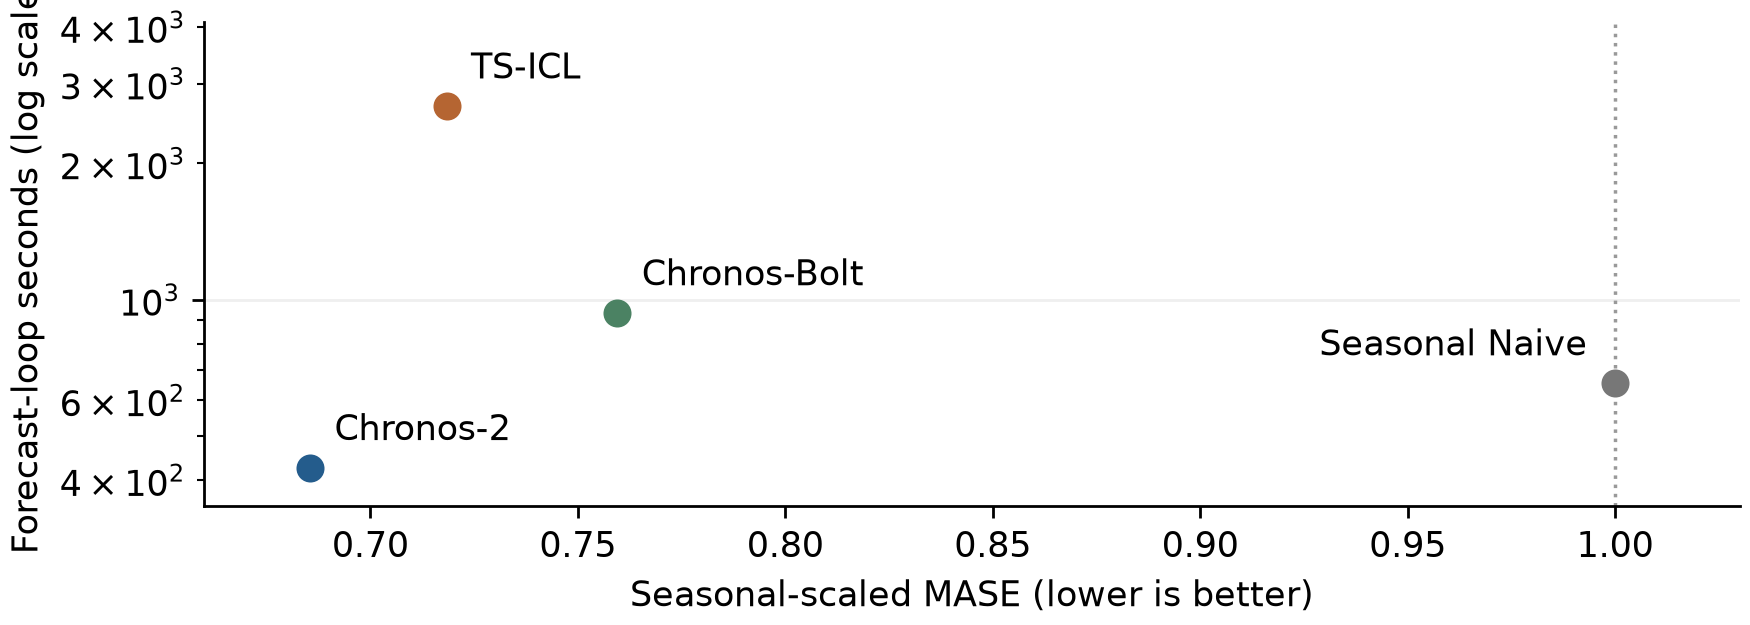
\includegraphics[width=0.93\linewidth]{executive_summary_accuracy_time.png}
\caption{Accuracy and total recorded forecast-loop time on the 98 tasks.
Lower and left is preferable. Time includes loop preparation but excludes
model loading, metric computation, and saving.}
\end{figure}

\textbf{Results.}
\begin{itemize}
\item Chronos-2's aggregate sMASE is \textbf{31.5\% better than Seasonal},
4.6\% better than TS-ICL, and 9.8\% better than Chronos-Bolt (lower error).
It leads on 74/98 tasks and
beats Seasonal on 48/50 configuration scores.
\item TS-ICL beats Chronos-2 on 21 tasks, and Chronos-Bolt on 8. These
pairwise counts differ from winning against \emph{both} competitors.
Their total forecasting times are 6.09 and 2.15 times Chronos-2's.
\end{itemize}

\textbf{Scope.} All three models complete all tasks, with 111,071 eligible
window--variate cells across items, out of 111,177 candidates. These are
metric cells, not future time steps. Context lengths and wrappers differ;
Seasonal uses CPU and learned models use accelerator inference. These
times are not hardware-independent backbone latencies.

\subsection*{Within-task error dispersion}
The task mean hides differences between forecast windows and channels.
Using the same eligible cells $G_k$, define the \textbf{population variance}
of task $k$'s cell errors for method $m$:
\[
 \operatorname{Var}_m(k)=\frac{1}{|G_k|}\sum_{c\in G_k}
 \left[\mase_m(c)-\overline{\mase}_m(k)\right]^2.
\]
The denominator is $|G_k|$, not $|G_k|-1$: these are descriptive statistics
of all evaluated cells, not estimates from repeated experimental runs.

For comparison with Seasonal Naive, define its variance on the same cells as
$\operatorname{Var}_{\mathrm{seasonal}}(k)$, using the formula above. The plot uses
\[
 \text{scaled mean}=\frac{\overline{\mase}_m(k)}{\mase_{\mathrm{seasonal}}(k)},
 \qquad
 \text{relative variance}=\frac{\operatorname{Var}_m(k)}{\operatorname{Var}_{\mathrm{seasonal}}(k)}.
\]
The second quantity is a ratio of variances, not the variance of scaled MASE.

\begin{figure}[h]
\centering
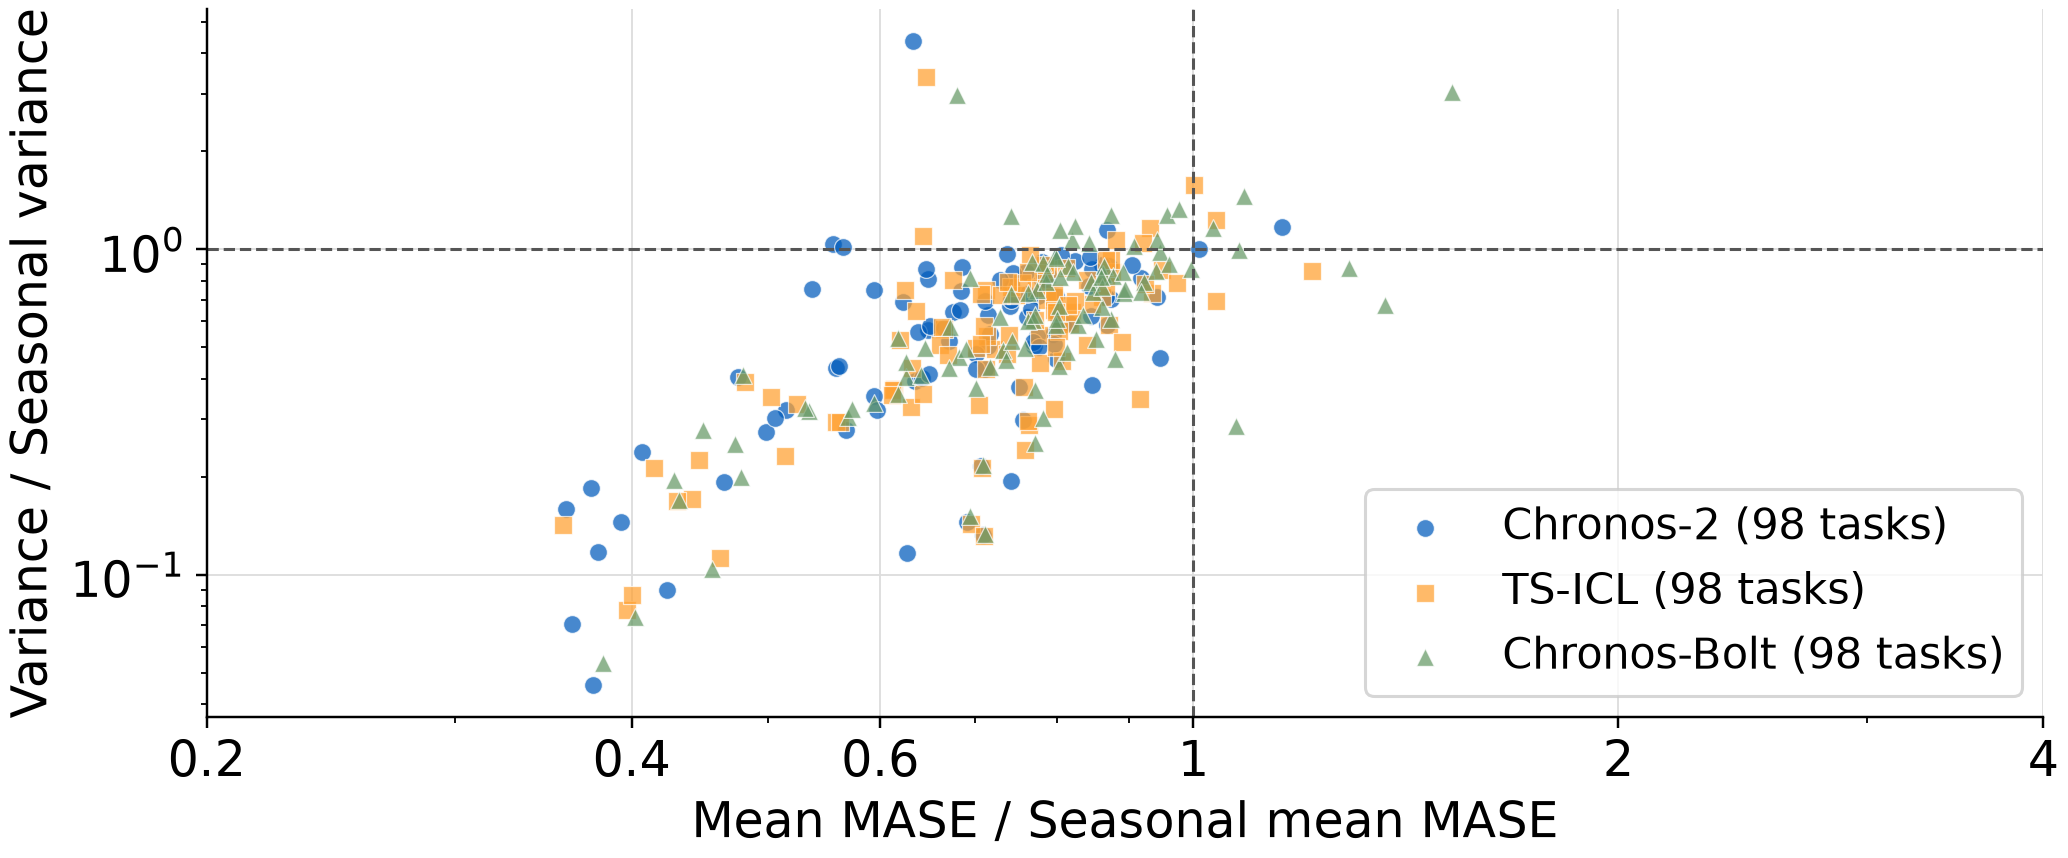
\includegraphics[width=\linewidth]{executive_summary_task_dispersion.png}
\caption{One point per selected model--task pair: \textbf{98 tasks per model,
294 points total}. The horizontal coordinate is the scaled task mean MASE;
the vertical coordinate is the population MASE variance divided by matched
Seasonal variance. Both axes are logarithmic and retain every point.
Dashed lines mark Seasonal parity at 1: left means better mean error, and
below means lower dispersion across windows and channels. Above 1 means
greater dispersion than Seasonal, not an invalid score.}
\end{figure}

\textbf{Observed dispersion.} Median variance ratios across the 98 tasks
are \textbf{0.590 for Chronos-2, 0.580 for TS-ICL, and 0.629 for
Chronos-Bolt}. Variance is lower than Seasonal on 93, 91, and 84 tasks,
respectively; both mean error and variance improve on 92, 89, and 80 tasks.
Chronos-2's lowest aggregate mean error therefore does not imply the lowest
median relative variance. The model clouds overlap, and some tasks have
greater dispersion than Seasonal. Lower variance alone does not guarantee
better forecasts: an error can be consistently large.

\newpage
\section{Chronos-2 channel representation}
\textbf{Question.} How does representing the same target histories jointly,
independently, or as past covariates affect accuracy and forecasting time?

For a multivariate window $x$, write $x_v$ for the history of variate $v$
and $x_{-v}$ for the histories of all other variates. The three modes are:
\begin{itemize}
\item \textbf{Native multivariate:} supply $x$ as one grouped target input,
and forecast all variates together.
\item \textbf{Independent univariate:} supply $x_v$ alone, separately for
each variate.
\item \textbf{Past-target covariates:} supply $x_v$ as the target and
$x_{-v}$ as past-only covariates, separately for each variate. This carries
the same historical information as native input through another interface;
no future values are supplied.
\end{itemize}

\textbf{Protocol.} All modes use frozen Chronos-2, the 8,192-step context
cap, at-most-16-item batches, identical quantiles, test windows, and Seasonal
support. The matched subset has \textbf{38 multivariate configurations and
74 tasks}. Its native score is not the 98-task foundation score.

\begin{table}[h]
\centering\small
\begin{tabularx}{\linewidth}{@{}Yrrrr@{}}
\toprule
Representation & sMASE & Change vs native & Seconds & Time ratio\\
\midrule
Native multivariate & 0.690045 & reference & 340.0 & 1.00\\
Independent univariate & 0.695590 & $+0.80\%$ & 350.2 & 1.03\\
Past-target covariates & 0.690045 & equivalent & 1,930.8 & 5.68\\
\bottomrule
\end{tabularx}
\caption{Matched 74-task sMASE and forecast-loop time. Positive score change
is worse. Time ratios divide total seconds by native total seconds.}
\end{table}

\begin{figure}[h]
\centering
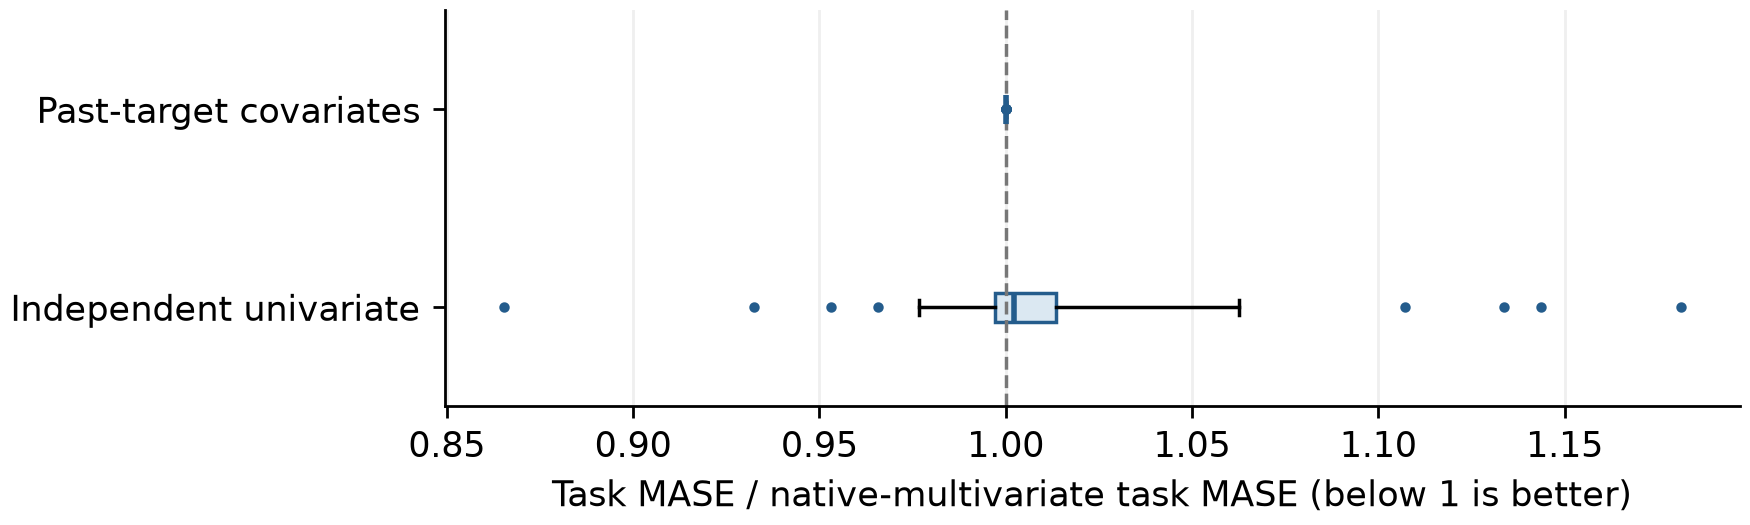
\includegraphics[width=0.93\linewidth]{executive_summary_channel_ratios.png}
\caption{Task MASE divided by matched native MASE, 74 ratios per mode.
Below 1 favors the alternative mode. Boxes show the middle 50\% and median;
whiskers span the 5th--95th percentiles, with remaining tasks shown as dots.
These distributions describe differences across tasks.}
\end{figure}

\textbf{Results and interpretation.}
\begin{itemize}
\item Native input wins 46 tasks and independent input wins 28. The
geometric mean independent/native ratio is 1.008; its middle-50\% task interval is
0.997--1.014. Native input's \textbf{0.8\% aggregate advantage is small
and varies across tasks}.
\item Past-target covariates reproduce native MASE: the largest absolute
relative difference is below $5.75\times10^{-7}$. They take \textbf{5.68
times the forecasting time}, without an accuracy gain in this comparison.
\end{itemize}
All modes complete all 74 tasks, using 91,319 eligible metric cells out
of 91,425 candidates.

\section{Dataset features associated with relative forecast error}
\textbf{Question.} Which measured dataset characteristics accompany higher
or lower sMASE across the evaluated configurations?

\textbf{Protocol.} Each model's configuration sMASE is paired with
full-series feature summaries, giving 50 configurations per model. Features
are computed per source variate and averaged over finite values within each
configuration. Spectral/decomposition preprocessing standardizes and
interpolates observations. STL (seasonal--trend decomposition by locally
estimated smoothing) uses the strongest detected candidate period, with a
nonseasonal smoothing fallback.

\textbf{Reported feature definitions.}
\begin{itemize}
\item \textbf{Temporal heterogeneity:} split a series into four chronological
blocks and average three components, each clipped to $[0,1]$:
\begin{itemize}
\item \emph{Location:} variance of block means divided by whole-series variance.
\item \emph{Scale:} $1-\exp(-\sigma^2)$, where $\sigma^2$ is the variance
of log block standard deviations relative to whole-series standard deviation,
regularized by $10^{-12}$.
\item \emph{Spectral:} mean base-2 Jensen--Shannon divergence between each
block's normalized power spectrum and the mean spectrum. This divergence
is mixture entropy minus mean individual entropy; spectra use 32 frequency
bins and a constant-signal bin. Series shorter than 16 steps receive zero
temporal heterogeneity.
\end{itemize}
\item \textbf{Spatial heterogeneity:} compare all source channels across
all series in a configuration, using each channel's full history, rather
than chronological blocks. ``Spatial'' here means differences between
channels, not geographic distance. Average three components clipped to $[0,1]$:
\begin{itemize}
\item \emph{Location:} variance of channel means divided by the sum of that
variance and the mean within-channel variance.
\item \emph{Scale:} $1-\exp(-\sigma^2)$, now with $\sigma^2$ the variance of
log channel standard deviations relative to their median standard deviation,
regularized by $10^{-12}$.
\item \emph{Spectral:} the same Jensen--Shannon comparison, between full-channel
spectra and their mean spectrum. A configuration with fewer than two source
channels has zero spatial heterogeneity.
\end{itemize}
\end{itemize}
Other feature names in the table link to their implementation or estimator.

\clearpage
\subsection*{Feature results and interpretation}
\begin{table}[H]
\centering\small
\begin{tabularx}{\linewidth}{@{}Yrrrr@{}}
\toprule
Feature & Chronos-2 & TS-ICL & Chronos-Bolt & Configs\\
\midrule
Temporal heterogeneity & $\mathbf{+0.497}$ & $\mathbf{+0.486}$ & $\mathbf{+0.418}$ & 50\\
Spatial heterogeneity & $-0.036$ & $-0.029$ & $+0.035$ & 50\\
\midrule
\href{https://raw.githubusercontent.com/Nixtla/tsfeatures/v0.4.5/tsfeatures/utils.py}{Trend Hurst} & $\mathbf{+0.438}$ & $\mathbf{+0.436}$ & $\mathbf{+0.360}$ & 50\\
Temporal scale heterogeneity & $\mathbf{+0.442}$ & $\mathbf{+0.418}$ & $+0.332$ & 50\\
Temporal location heterogeneity & $+0.409$ & $+0.397$ & $\mathbf{+0.369}$ & 50\\
\midrule
\featurecode{179}{Second detected period} & $\mathbf{-0.429}$ & $\mathbf{-0.368}$ & $\mathbf{-0.332}$ & 39\\
\featurecode{569}{Seasonal strength} & $\mathbf{-0.352}$ & $-0.254$ & $-0.132$ & 50\\
\featurecode{536}{Seasonal cycle correlation} & $\mathbf{-0.280}$ & $-0.202$ & $-0.168$ & 50\\
\featurecode{578}{Stationarity} & $-0.128$ & $\mathbf{-0.280}$ & $-0.242$ & 50\\
\href{https://raw.githubusercontent.com/Nixtla/tsfeatures/v0.4.5/tsfeatures/tsfeatures.py}{Spectral entropy} & $-0.192$ & $\mathbf{-0.277}$ & $\mathbf{-0.356}$ & 50\\
\featurecode{637}{Spikiness} & $-0.166$ & $-0.142$ & $\mathbf{-0.272}$ & 50\\
\bottomrule
\end{tabularx}
\caption{Spearman rank correlations with configuration sMASE: Pearson
correlation of ranks, assigning average ranks to ties. Bold entries are each
model's top three positive or top three negative correlations among all
extracted features; rows are their union plus spatial heterogeneity. Positive
means larger features accompany worse relative error. Counts use pairwise
finite configurations.}
\end{table}

\begin{figure}[H]
\centering
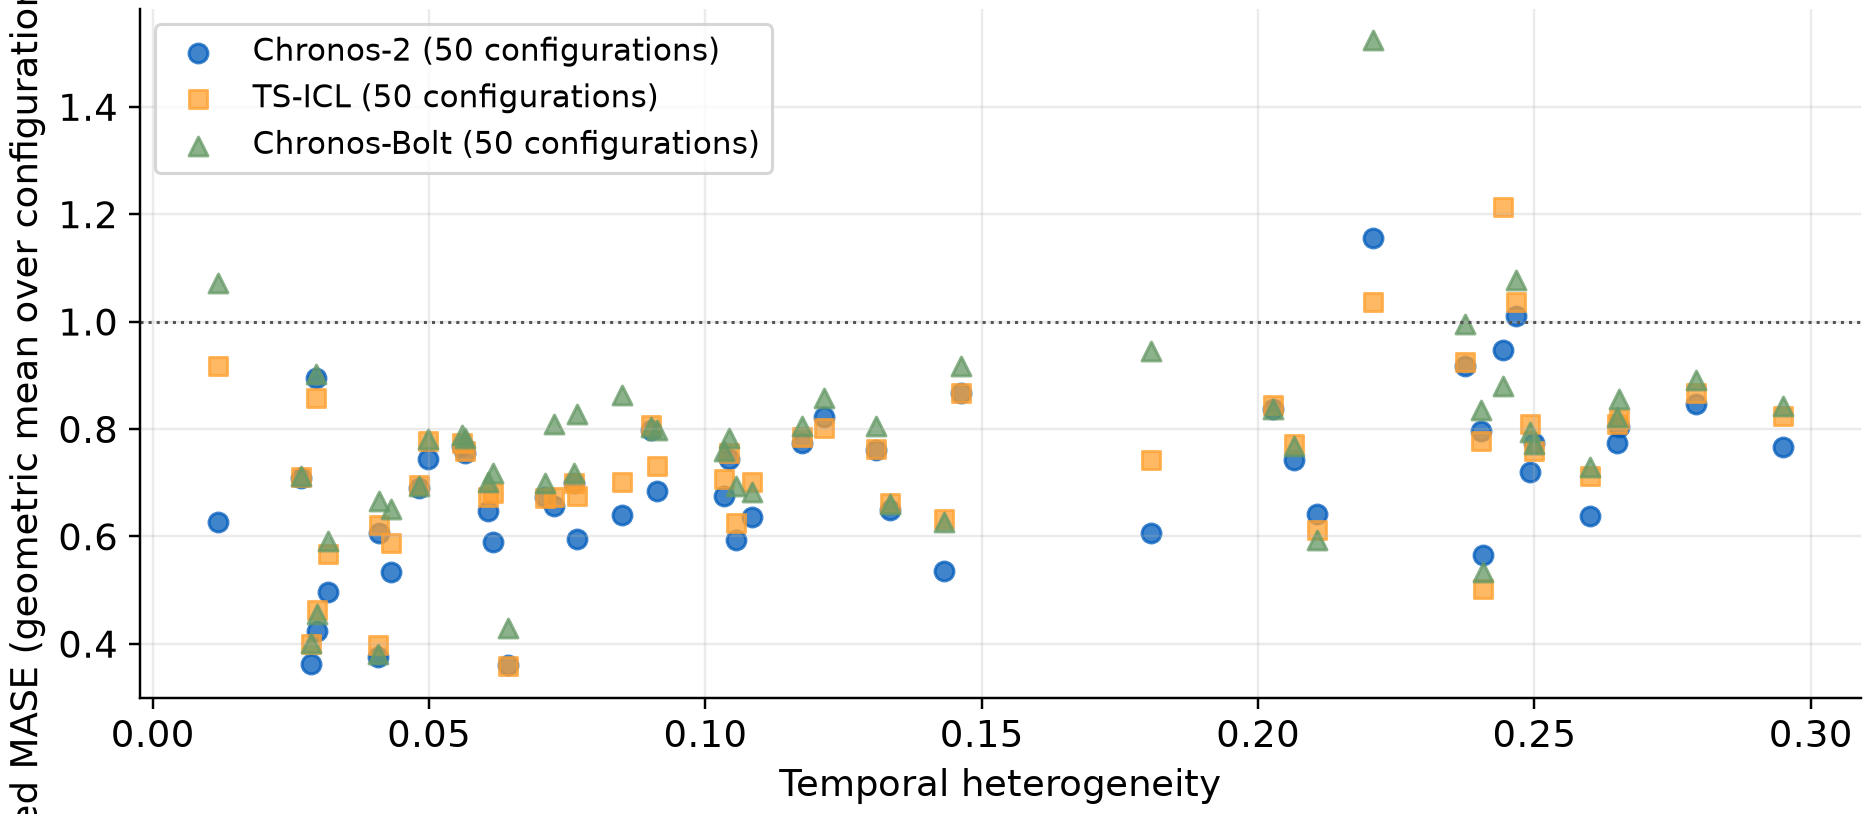
\includegraphics[width=0.65\linewidth]{executive_summary_feature_scatter.png}
\caption{Temporal heterogeneity versus configuration sMASE, replotted from
the completed feature-analysis data: 50 points per model in one panel. The
dotted line marks Seasonal parity.}
\end{figure}

\textbf{Interpretation.} Greater temporal heterogeneity and trend Hurst
accompany worse relative forecast error for all three models. Spatial
heterogeneity has near-zero correlations ($-0.036$ to $+0.035$), unlike
temporal heterogeneity. Negative leaders vary by model: second detected
period, seasonal strength/correlation, stationarity, spectral entropy,
and spikiness.
These cross-dataset associations do not isolate causal effects. The displayed
features were selected from the extracted feature set and use full series,
including test observations, so they describe the obtained errors rather than
an evaluated pre-forecast model-selection rule.

\textbf{Evidence scope.} Selected task records and metric summaries were
checked; raw arrays were not. The IQRs and correlations describe this
benchmark, not repeated-run variability.

\clearpage
\section{Maximum input context length}
\textbf{Question.} How much history should each frozen forecaster receive?
Longer inputs may improve accuracy but increase inference work. The tested
factor is the maximum retained input length, not the forecast horizon.

\textbf{Protocol.} For each of Chronos-2, Chronos-Bolt, and TS-ICL, the
model-specific maximum is successively halved four times. Each of the 15
model--context settings completes the same 98 TIME tasks on the same 111,071
eligible window--channel cells. The input at each forecast origin is the
most recent available history up to the selected cap; shorter histories
remain shorter. Model weights, output quantiles, official test windows,
Seasonal support, and sMASE aggregation are unchanged. There is one selected
run per setting, not repeated-seed uncertainty.

\begin{figure}[H]
\centering
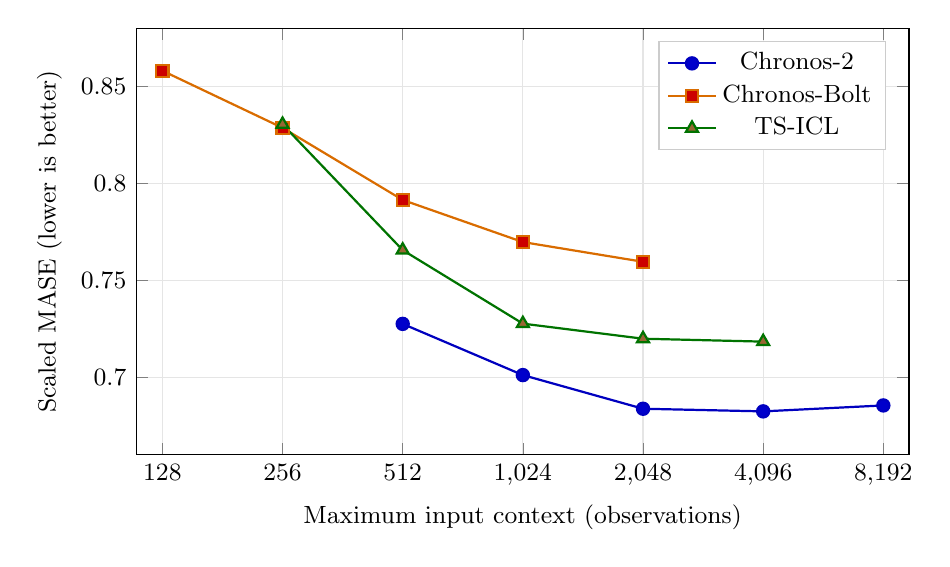
\begin{tikzpicture}
\begin{axis}[
  width=0.94\linewidth,height=7cm,
  xmode=log,log basis x=2,
  xmin=110,xmax=9500,ymin=0.66,ymax=0.88,
  xtick={128,256,512,1024,2048,4096,8192},
  xticklabels={128,256,512,1{,}024,2{,}048,4{,}096,8{,}192},
  xlabel={Maximum input context (observations)},
  ylabel={Scaled MASE (lower is better)},
  grid=major,grid style={gray!20},
  legend pos=north east,
  legend style={font=\small,draw=gray!40,fill=white},
  tick label style={font=\small},
  label style={font=\small},
]
\addplot+[blue!75!black,thick,mark=*,mark size=2.2pt] coordinates {
  (512,0.7275443013) (1024,0.7011391104) (2048,0.6837876399)
  (4096,0.6824273666) (8192,0.6854886145)};
\addlegendentry{Chronos-2}
\addplot+[orange!85!black,thick,mark=square*,mark size=2.2pt] coordinates {
  (128,0.8580839526) (256,0.8286274292) (512,0.7914364011)
  (1024,0.7697317055) (2048,0.7595590358)};
\addlegendentry{Chronos-Bolt}
\addplot+[green!45!black,thick,mark=triangle*,mark size=2.5pt] coordinates {
  (256,0.8304099842) (512,0.7655854536) (1024,0.7276728542)
  (2048,0.7198958692) (4096,0.7183939833)};
\addlegendentry{TS-ICL}
\end{axis}
\end{tikzpicture}
\caption{Aggregate sMASE versus maximum input context for each frozen model.
Each point is the geometric mean of 98 Seasonal-scaled task MASE ratios on
the shared evaluation grid; lines connect only the five tested settings per
model and do not establish behavior between them. Context is on a base-2
logarithmic axis; lower sMASE is better.}
\end{figure}

\textbf{Results.} Chronos-2 at 4,096 steps improves aggregate sMASE by
0.45\% and reduces recorded time by 40.7\% relative to 8,192. At 2,048
steps, its sMASE is still 0.25\% lower, with 63.9\% less time. The paired
4,096-versus-8,192 comparison improves 49 tasks, ties exactly on 28, and
worsens 21; its median task change is only $-0.01\%$. Thus the aggregate
advantage is modest and not uniform. Chronos-Bolt and TS-ICL attain their
lowest sMASE at the longest tested context. Halving that context worsens
their aggregate scores by 1.34\% and 0.21\%, respectively, while reducing
recorded time by 38.9\% and 59.5\%. Their shortest settings worsen sMASE
by 12.97\% and 15.59\% relative to their maxima.

\textbf{Limit.} Each timing is a single-launch forecast-loop total, not a
controlled repeated latency estimate or an end-to-end job duration. The
comparison supports a model-specific accuracy--cost tradeoff on these tasks,
not a universal optimal context length.

\clearpage
\section{Per-instance input z-score normalization}
\textbf{Question.} Does centering and scaling each retained input window
improve frozen-model accuracy when forecasts are returned to the target's
original units?

\textbf{Protocol.} Compare unchanged input with z-scored input for each of
the three models at its maximum context (8,192, 2,048, and 4,096 steps,
respectively). For each window and variate, compute the finite-value mean
and population standard deviation along time after context truncation;
constant finite inputs use unit scale. Missing positions remain missing.
Every predicted quantile is inverse-transformed before scoring. Each of the
six model--mode settings completes the same 98 tasks and 111,071 eligible
cells. The unchanged-input arms exactly reproduce the matching task metric
summaries from the maximum-context evaluation.

\begin{table}[h]
\centering\small
\begin{tabular}{@{}lrrrr@{}}
\toprule
 & \multicolumn{2}{c}{sMASE $\downarrow$} & \multicolumn{2}{c}{Forecast-loop seconds $\downarrow$}\\
Model & Unchanged & Z-score & Unchanged & Z-score\\
\midrule
Chronos-2 & 0.685488615 & 0.685488629 & 434.6 & 431.7\\
TS-ICL & 0.718393983 & 0.718393972 & 2,681.1 & 2,686.8\\
Chronos-Bolt & 0.759559036 & 0.759558465 & 945.6 & 1,001.6\\
\bottomrule
\end{tabular}
\caption{Matched 98-task geometric sMASE per model and mode. Seconds are
single-launch forecast-loop totals, not a controlled speed comparison.}
\end{table}

\textbf{Result and interpretation.} Z-scoring provides no material aggregate
accuracy gain for these frozen models on this benchmark. Every model's two
scores agree to at least five decimal places, and the largest relative
difference on any paired task is 0.0061\%. This near-invariance concerns the
tested input/output transformation; it does not imply all normalization
methods are interchangeable. An entirely missing retained window has no
finite mean or scale and remains non-finite rather than receiving an invented
signal; the completed selected tasks provide no evidence of such a window
reaching a model. Timing differences from one launch do not establish a
normalization speed effect.
\end{document}
